\subsection{Линейное программирование --- геометрический метод.}
\begin{example}
	\begin{equation*}
		f=x_1+2x_2 \to \max
	\end{equation*}
	\begin{equation*}
		\begin{cases}
			4x_1-2x_2\leq12\\
			-x_1+3x_2\leq6\\
			2x_1+4x_2\geq16\\
			x_1,x_2\geq0
		\end{cases}
	\end{equation*}
	\begin{solution}
		\textbf{1. Найдем градиент функции.}
		\begin{equation*}
			\overline{\operatorname{grad}}f=(1,2)
		\end{equation*}
		\begin{figure}[H]
			\centering
			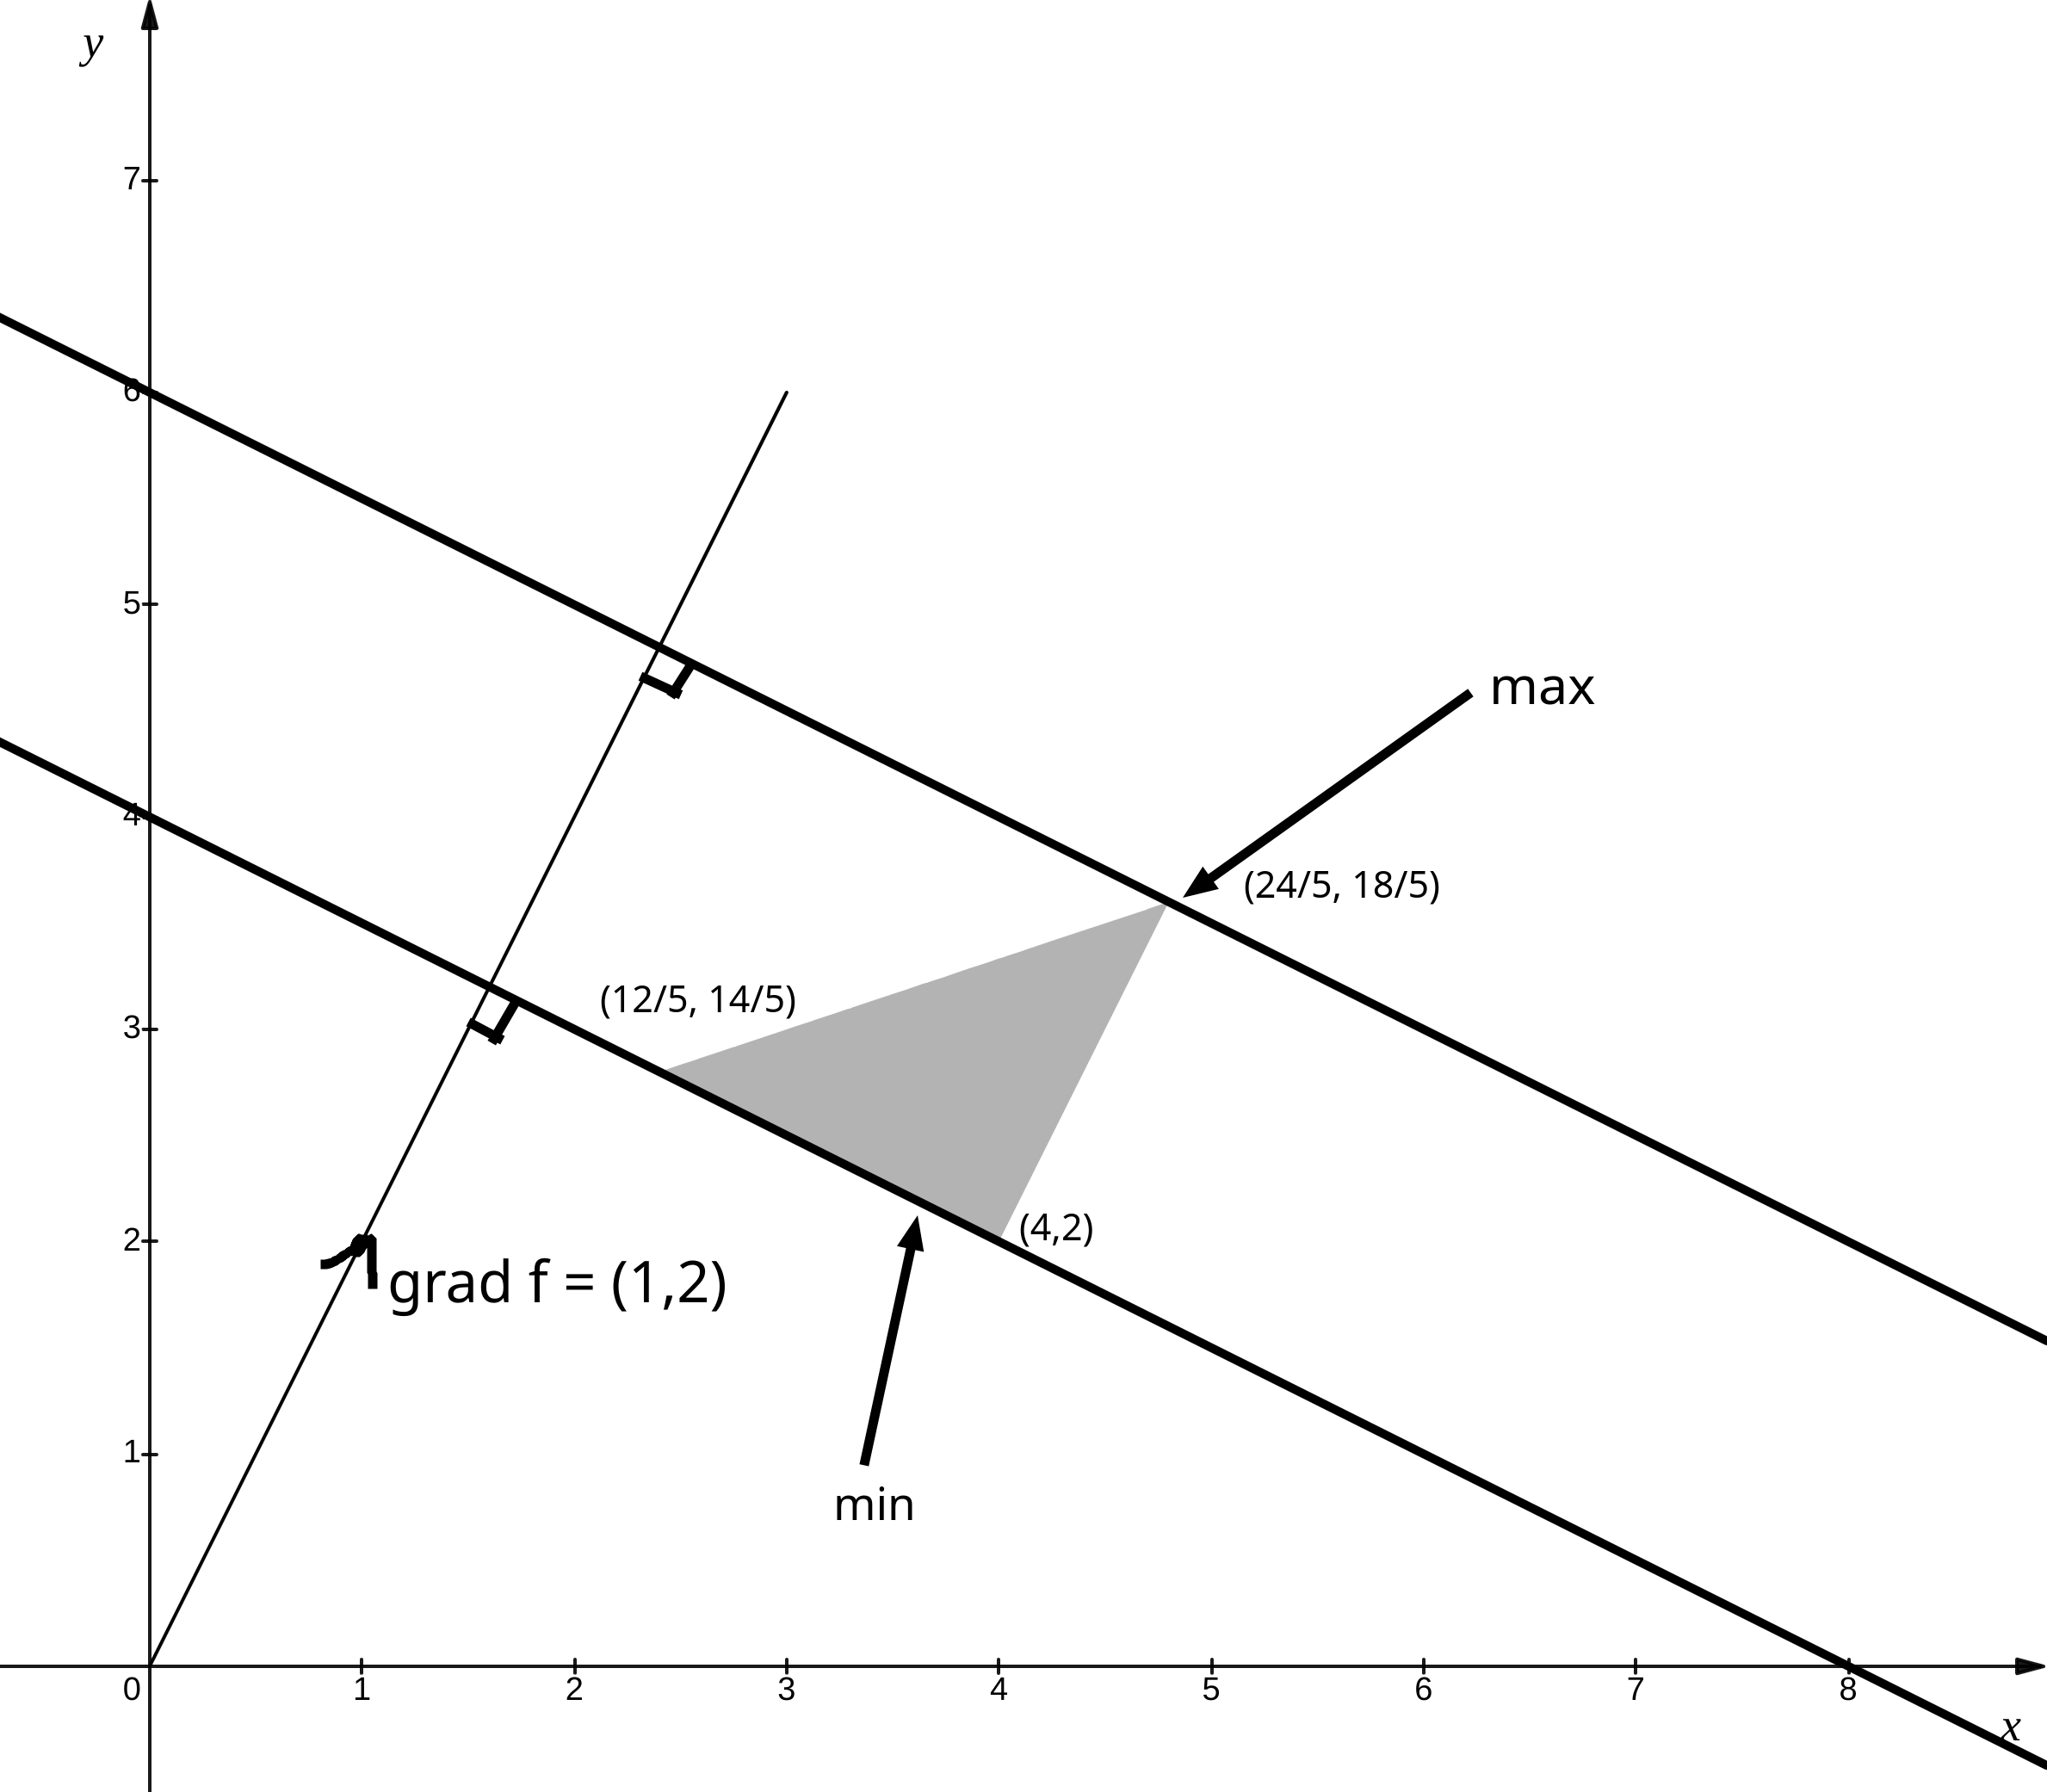
\includegraphics[width=0.7\linewidth]{img/prac4}
			\caption{}
			\label{fig:prac4}
		\end{figure}
		Рассмотрим прямую
		\begin{equation*}
			\overline{\operatorname{grad}}f\cdot\left(\begin{matrix}
				x_1\\
				x_2
			\end{matrix}\right) = x_1 + 2x_2 = C \Rightarrow x_2=-\frac{x_1}{2} + \frac{C}{2}
		\end{equation*}
		Будем двигать ее параллельным переносом, тогда получим следующее:
		
		Максимальное значение функции
		\begin{equation*}
			(\dfrac{24}{5},\dfrac{18}{5})\Rightarrow \boxed{C=12}
		\end{equation*}
		Минимальное значение функции
		\begin{equation*}
			(4, 2)\Rightarrow \boxed{C=8}
		\end{equation*}
	\end{solution}
\end{example}